\documentclass[11pt,a4paper]{article}
\usepackage{graphicx}
\graphicspath{{images/}}
\begin{document}
\section{Figures}
Figure~\ref{fig:plot} is a PNG at its natural size, two inches wide at
300 dots per inch, and Figure~\ref{fig:bars} is a JPEG scaled to half the
line width.

\begin{figure}[h]
\centering
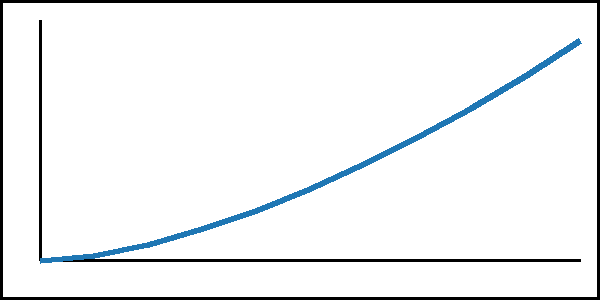
\includegraphics{plot}
\caption{A plot at its natural size.}\label{fig:plot}
\end{figure}

Text continues after the first figure and is long enough to wrap onto a
second line, so the spacing after a figure can be measured.

\begin{figure}[h]
\centering
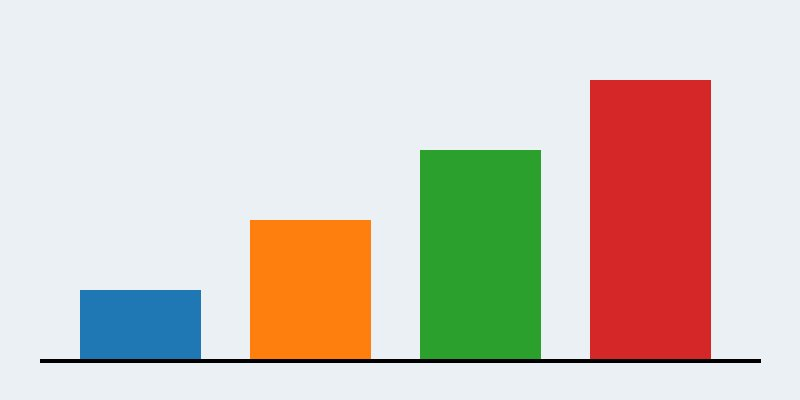
\includegraphics[width=0.5\linewidth]{bars.jpg}
\caption{A bar chart scaled to half the line width.}\label{fig:bars}
\end{figure}

After both figures the text continues.
\end{document}
